\documentclass[a4paper]{article}

\usepackage[english]{babel}
\usepackage[utf8]{inputenc}
\usepackage{amsmath}
\usepackage{graphicx}
\usepackage[colorinlistoftodos]{todonotes}
\usepackage{indentfirst}
\usepackage{url}
\usepackage{listings}
\usepackage{xcolor}
\usepackage{float}
\usepackage{algorithm}  
\usepackage{algpseudocode}  
\renewcommand{\algorithmicrequire}{\textbf{Input:}}  % Use Input in the format of Algorithm  
\renewcommand{\algorithmicensure}{\textbf{Output:}} % Use Output in the format of Algorithm  
\setlength{\parindent}{2em}

\title{MLP Machine Learning Method in Finance Engineering}

\author{Xinzhe Li and Fengyuan Jia}

\date{2018 Fall}

\begin{document}
\maketitle

\begin{abstract}
The report is going to represent reader the basic algorithm of Multi-Layer Perceptron(MLP) and a MLP library written in C++ along with its two supporting libraries, numpy library and activation library. Two tests were delivered to show the usability of the libraries. The introduction and usage method of library APIs are also included. 

Workload:

Xinzhe Li:   Libraries Implementation, Model Testing, Report

Fengyuan Jia:   Data Collecting, Read Data Function Implementation  
\end{abstract}

\section{Preliminary}
\label{sec:introduction}
\subsection{What is Machine Learning?}
Machine learning (ML) is the study of algorithms and mathematical models that computer systems use to progressively improve their performance on a specific task. Machine learning algorithms build a mathematical model of sample data, known as "training data", in order to make predictions or decisions without being explicitly programmed to perform the task.\cite{nano3}

Machine learning algorithms are used in the applications of email filtering, detection of network intruders, and computer vision, where it is infeasible to develop an algorithm of specific instructions for performing the task. It is a useful tool. The MLP library represented by this report is a class of feedforward artificial neural network, a subsection of machine learning. 
\subsection{Why we need Machine Learning?}

Machine learning can play an important role in industries which work with massive data. We list several benefits below:

\begin{itemize}
	\item{\textbf{Processing big data}}
    \item{\textbf{Learning and expressing relationships between features automatically} }
    \item{\textbf{Regression/Classification problems} }
    \item{\textbf{Linear/Nolinear problems} }
    \item{\textbf{Supervised/Unsupervised problems} }
\end{itemize}

\section{Data Selection}
\label{sec:theory}

\subsection{Data Source}
It is difficult to implement crawler in C++ to fetch data from Internet automatically. So we use some ready-made clean data to test the workability of our model. 


We use the data from https://challenger.ai/competition/trendsense/subject, it is an AI challenge competition which provide stocks data for us to check our model’s/APIs' ability.

\subsection{Data Explanation}

There are 87 features in the provided data set, we won’t use the weight column, era column and the group column (Table 1). 

We guess that not all features are necessary. These features may in different types, such as fundamentals, technology, finance, Greek and some others. But it is hard to tell which one is useless. It is true that training the model in variable types of the data with less repetition is a good choice. So under this circumstance, we can either manually choose 1 feature in each 10 (less or more) features (proposed by Fengyuan Jia) or give all features to the model, asking model to figure out and express the relationship between them (proposed by Xinzhe Li).    
\begin{table}[H]
\centering
\begin{tabular}{|c|c|c|c|}
 \hline
feature84& feature85& feature86& feature87 \\
 \hline
1.514802873 & -0.859637483 & -0.838864073 &-1.697329532  \\
 \hline
weight& label& group& era\\
  \hline
10 & 1&11&1\\
\hline
\end{tabular}\\
\caption{\label{tab:widgets}Data Example Table.}
\end{table}

\subsection{Model Application}
The model/APIs was implemented for supervised classification problems. So users who want to use the model must provide data contain both label and features. 


1.First,you can use crawler to collect from Yahoo finance or API in Bloombery and IB data. Generate binary label (0 and 1) from data according to your need (for example: calculate ups and downs, 1 stands for up, 0 stands for down) or use the label provided by supplier. And save data and label into the local file.


2.Second, if your data is not ready-made and clean, you need to format it and delete the extreme data of features. Normalize the data. Then check the correlations between your features and select suitable features.

The Skipped Huber Method:
\[ D{i,upper} = D_m +5.2D_{MAD},     \ if \ D_i \geq D_m+5.2D_{MAD} \]
\[ D{i,lower} = D_m -5.2D_{MAD},     \ if \ D_i \leq D_m+5.2D_{MAD} \]

normalized:\[ (D_i-E_D)/STD\]

\subsection{Strategy Building}
A label tells the machine to be or not to be. For training data, the stock worth to buy has a label of 1, others have a label of 0. The model learns from training data to represent under what circumstances stocks are worth to buy and under what are not. After training model can tell whether to buy or not when new circumstances are provided. In the true world trade, you need to change your positions depending on model forecast (label:0 or 1) as the time goes by. 


Finally, it is not necessary to use the data long ago to train the model. History data may not be sufficient enough to represent nowadays’ market condition. So, update the knowledge of the model per period by training it with new data.

\section{Main Work}
This section will cover the theory foundation and implementation details of three main libraries.   

\subsection{numpy Library}
The name of the numpy library comes from a Python library called NumPy. NumPy is the fundamental package for scientific computing with Python.\cite{nano2} It contains among other things:

\begin{itemize}
	\item{\textbf{A powerful N-dimensional array object}}
    \item{\textbf{Sophisticated (broadcasting) functions} }
    \item{\textbf{Useful linear algebra, Fourier transform, and random number capabilities} }
\end{itemize}

Programmer of the group implemented some of the features mentioned above, to fit the need of matrix operations and calculations in machine learning algorithms.    


\subsubsection{Implement Details}
The library aims to provide basic matrix operations and calculations. it simulates some of the functions from NumPy library. Operations including reshaping, random generating matrix value. Calculations including addition (matrix and matrix or matrix and double), division (matrix and double/int), star product (matrix and matrix), dot product (matrix and matrix), subtraction (matrix and double/int).

\subsubsection{APIs}                                                                    
This section shows and explains some of important APIs from numpy library.\\\\
\textbf{\Large Randomly Initial}\\           
\begin{lstlisting}[language={[ANSI]C++},keywordstyle=\color{blue!70},commentstyle=\color{red!50!green!50!blue!50},frame=shadowbox, rulesepcolor=\color{red!20!green!20!blue!20}]
numpy(const double low, const double high, const int row, 
const int col)
\end{lstlisting}

The construction function randomly initializes value of elements in a matrix with a given bounded.

\textbf{Arguments}
\begin{itemize}
	\item{\textbf{low:} Lower bound of randomly initial value}
    \item{\textbf{high:} Upper bound of randomly initial value}
    \item{\textbf{row:} Number of row of numpy matrix}
    \item{\textbf{col:} Number of column of numpy matrix}
\end{itemize}
\textbf{\Large Start Product(*)}\\
\begin{lstlisting}[language={[ANSI]C++},keywordstyle=\color{blue!70},commentstyle=\color{red!50!green!50!blue!50},frame=shadowbox, rulesepcolor=\color{red!20!green!20!blue!20}]
numpy operator *(numpy &m1, numpy &m2)
\end{lstlisting}

The function implements elementwise product. The matrixes must be in the same shape\\\\
\textbf{\Large Dot Product}\\
\begin{lstlisting}[language={[ANSI]C++},keywordstyle=\color{blue!70},commentstyle=\color{red!50!green!50!blue!50},frame=shadowbox, rulesepcolor=\color{red!20!green!20!blue!20}]
numpy dot(numpy &m1, numpy &m2)
\end{lstlisting}

The function implements matrix product. \\\\
\textbf{\Large Reshape}\\
\begin{lstlisting}[language={[ANSI]C++},keywordstyle=\color{blue!70},commentstyle=\color{red!50!green!50!blue!50},frame=shadowbox, rulesepcolor=\color{red!20!green!20!blue!20}]
void reshape(int row, int col)
\end{lstlisting}

The function can reshape a m*n numpy matrix to a l*r numpy matrix as long as m*n = l*r.\\

\subsection{Activation Function Library}
In artificial neural networks, the activation function of a node defines the output of that node, or "neuron," given an input or set of inputs. This output is then used as input for the next node and so on until a desired solution to the original problem is found\cite{nano1}.
\subsubsection{Implement Details}
Five most used activation functions were implemented in the library. Their parameters can be double or self-defined object numpy.

\textbf{Sigmod}
$$f(x)=\frac{1}{1+e^{-x}}$$
\begin{figure}[H]
\centering
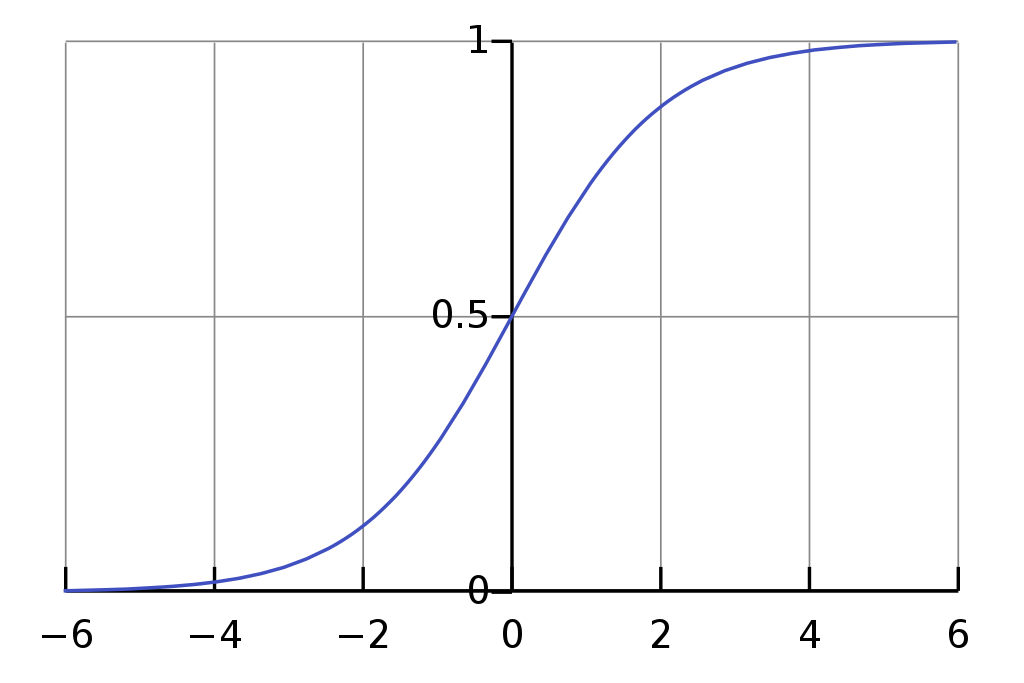
\includegraphics[width=0.5\textwidth]{sigmod.png}
\caption{\label{fig:frog}Sigmod}
\end{figure}

\textbf{Tanh}
$$f(x)=\frac{e^{x}-e^{-x}}{e^{x}+e^{-x}}$$
\begin{figure}[H]
\centering
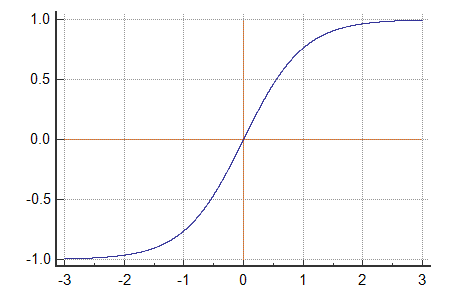
\includegraphics[width=0.5\textwidth]{tanh.png}
\caption{\label{fig:frog}TanH}
\end{figure}

\textbf{Rectified linear unit (ReLU)\cite{nano4}}
$$f(x)=\left\{\begin{matrix}
0 & for\ x< 0\\ 
 & \\ 
x & for\ x\geq 0 
\end{matrix}\right.$$
\begin{figure}[H]
\centering
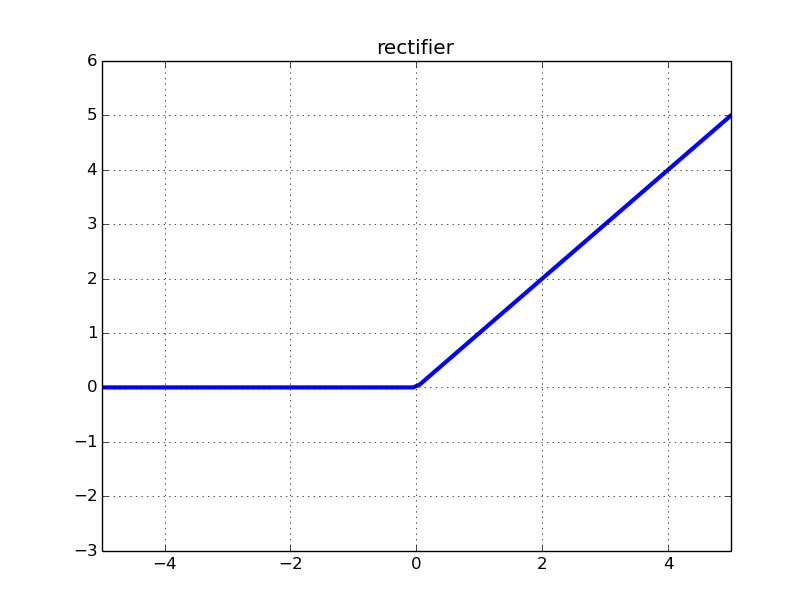
\includegraphics[width=0.5\textwidth]{RELU.png}
\caption{\label{fig:frog}ReLU}
\end{figure}

\textbf{Parameteric rectified linear unit (PReLU)\cite{nano5}}
$$f(\alpha ,x)=\left\{\begin{matrix}
\alpha x & for\ x< 0\\ 
 & \\ 
x & for\ x\geq 0 
\end{matrix}\right.$$
\begin{figure}[H]
\centering
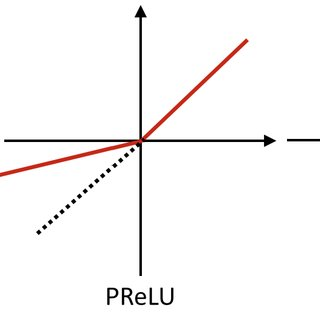
\includegraphics[width=0.5\textwidth, height=0.35\textwidth]{PRELU.jpg}
\caption{\label{fig:frog}PReLU}
\end{figure}
\textbf{Exponential linear unit (ELU)\cite{nano6}}
$$f(\alpha ,x)=\left\{\begin{matrix}
\alpha (e^{x}-1) & for\ x\leq  0\\ 
 & \\ 
x & for\ x>  0 
\end{matrix}\right.$$
\begin{figure}[H]
\centering
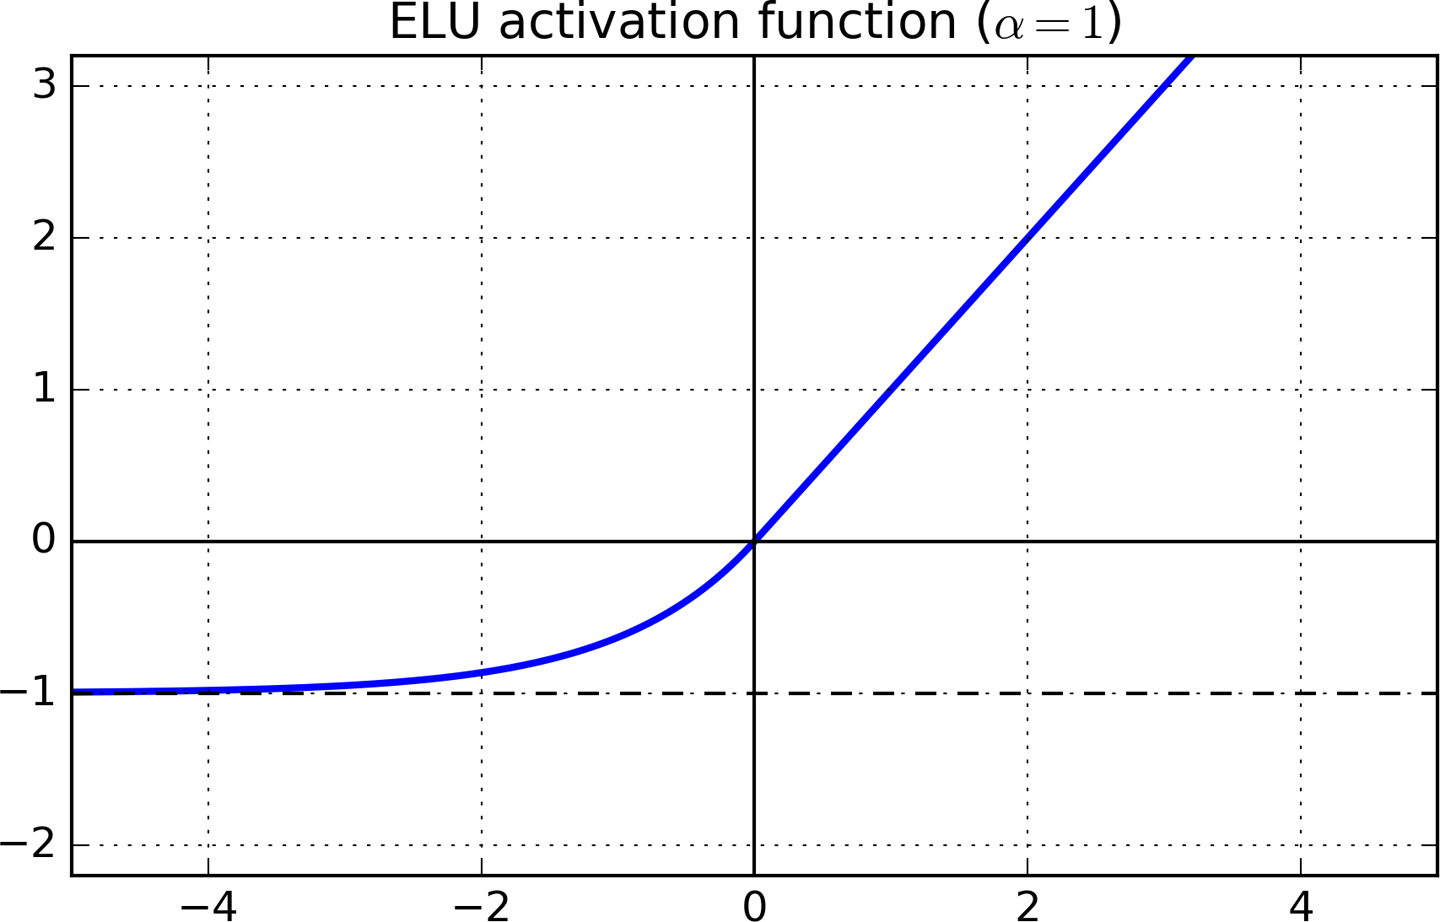
\includegraphics[width=0.5\textwidth]{ELU.png}
\caption{\label{fig:frog}ELU}
\end{figure}
\subsection{MLP Library}
\subsubsection{Basic Algorithm}
A multilayer perceptron (MLP) is a class of feedforward artificial neural network. An MLP consists of, at least, three layers of nodes: an input layer, a hidden layer and an output layer. Nodes on layers are fully connected with nodes on other layers by connection weight. And each layer expect input layer has bias of its own. Except for the input nodes, each node is a neuron that uses a nonlinear activation function. MLP utilizes a supervised learning technique called backpropagation for training.\cite{nano7}\cite{nano8} Its multiple layers and non-linear activation distinguish MLP from a linear perceptron. It can distinguish data that is not linearly separable.\cite{nano9}
\begin{figure}[H]
\centering
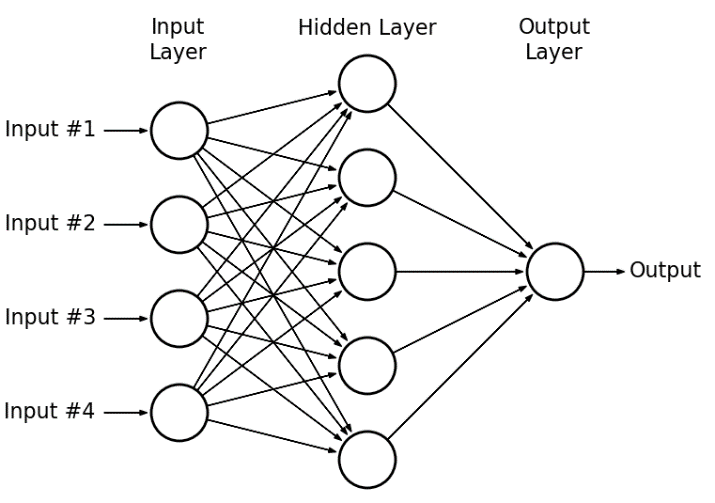
\includegraphics[width=0.5\textwidth]{MLP.png}
\caption{\label{fig:frog}An Example of MLP}
\end{figure}
Learning occurs in the perceptron by changing connection weights and bias after each piece of data is processed. The goal of training is getting a better expression of the given problem which means to maximize log likelihood function:
$$\overrightarrow{w} = \arg\max_{\overrightarrow{w}}\ln\prod_iP(y_i|x_i;\overrightarrow{w})$$
or to minimize loss function by updating connection weight and bias:
$$\overrightarrow{w} = \arg\min_{\overrightarrow{w}}\sum_i \frac{1}{2}(y_i-\widehat{f}(x_i;\overrightarrow{w}))^2$$

In MLP, it is achieved using gradient descent algorithm. $\overrightarrow{w}$ stands for connection weight, $\eta$ stands for learning rate and $ \eta \bigtriangledown E_{D}[\overrightarrow{w}]$ stands for gradient of $\overrightarrow{w}$:
$$\overrightarrow{w} = \overrightarrow{w} - \eta \bigtriangledown E_{D}[\overrightarrow{w}]$$

The core part of gradient descent is calculating gradient. Forward propagation and back propagation are being used. For forward propagation, test data put into network and get a observed output $o_{d}$ from network. And back propagation basing on the $o_{d}$ and $y_{d}$, the target output of the data (label of the data), to calculate gradient using formula below:\\
$$\Delta \overrightarrow{w} =  - \eta \bigtriangledown E_{D}[\overrightarrow{w}]$$\\
$$\Delta w_{i} =  - \eta \frac{\partial E}{\partial w_{i}}$$\\
$$\frac{\partial E[\overrightarrow{w}]}{\partial w_{j}} =   \frac{\partial }{\partial w_{i}}\frac{1}{2} \sum_{d}(t_{d}-o_{d})^{2}$$\\
$$=   \frac{1}{2} \sum_{d} 2(t_{d}-o_{d})\frac{\partial }{\partial w_{i}}(t_{d}-o_{d})$$
$$=   \sum_{d} (t_{d}-o_{d})(-\frac{\partial o_{d}}{\partial w_{i}})$$\\
$$=   \sum_{d} (t_{d}-o_{d})\frac{\partial o_{d}}{\partial net_{i}}\frac{\partial net_{i}}{\partial w_{i}}$$\\
$$=   -\sum_{d} (t_{d}-o_{d})o_{d}(1-o_{d})x_{d}^i$$\\
$$:where \ net=   \sum_{i=0}^{n} w_{i}x_{i}$$\\

After the gradient calculated, there are two modes to update weight: Batch Mode and Incremental Mode.
\begin{algorithm}[H]  
  \caption{Batch Mode}  
  \label{alg::conjugateGradient}  
  \begin{algorithmic}[1]  
    \Repeat  
      \State compute gradient $\bigtriangledown E_{D}[\overrightarrow{w}]$;  
      \State $\overrightarrow{w} = \overrightarrow{w} - \eta \bigtriangledown E_{D}[\overrightarrow{w}]$  
    \Until{converge}  
  \end{algorithmic}  
\end{algorithm} 
 \begin{algorithm}[H]  
  \caption{Incremental Mode}  
  \label{alg::conjugateGradient}  
  \begin{algorithmic}[1]  
    \Repeat  
      \For{for each training example d in D}  
       \State compute gradient $\bigtriangledown E_{d}[\overrightarrow{w}]$;  
       \State $\overrightarrow{w} = \overrightarrow{w} - \eta \bigtriangledown E_{D}[\overrightarrow{w}]$  
      \EndFor 
    \Until{converge}  
  \end{algorithmic}  
\end{algorithm}

Our library uses Batch Mode to update connection weight. 
\subsubsection{Implement Details}
The first step to start a MLP is initializing connection weight and bias matrices. The dimensions of weight and bias are related to input , output dimensions and number of neurons on the layer. In our library, the output dimension is one and input dimension decided by input (in machine learning context a piece of data with n features has n dimensions, it is different from dimensions in geometry context). The MLP has three layers: one input layer, one hidden layer and one output layer. The value of the weights and biases are randomly generated and bounded by the bound defined by input dimensions and number of neurons in hidden layer. The bound follows the formula:

$$upperbound = \sqrt{\frac{6}{input\ dimension + hidden\ layer\ neuron\ number}}$$
$$lowerbound = -\sqrt{\frac{6}{input\ dimension + hidden\ layer\ neuron\ number}}$$
\begin{lstlisting}[language={[ANSI]C++},,keywordstyle=\color{blue!70},commentstyle=\color{red!50!green!50!blue!50},frame=shadowbox, rulesepcolor=\color{red!20!green!20!blue!20}, title={Initialization},  basicstyle=\footnotesize, numbers=left]  
double low=-sqrt(6.0/(x_train.columns()+this->hidden_layer_size));
double high=sqrt(6.0/(x_train.columns()+this->hidden_layer_size));

this->w1=numpy(low,high,this->hidden_layer_size,x_train.columns());
this->w2=numpy(low,high,1,this->hidden_layer_size);
this->b1=numpy(low,high,this->hidden_layer_size,1);
this->b2=numpy(low,high,1,1);
\end{lstlisting} 

The forward propagation inputs training data into the MLP to calculate the current output. The library can only use sigmod function as the activate function so far. Choosing activate function by sending parameter to object is not included.
\begin{lstlisting}[language={[ANSI]C++},,keywordstyle=\color{blue!70},commentstyle=\color{red!50!green!50!blue!50},frame=shadowbox, rulesepcolor=\color{red!20!green!20!blue!20}, title={Forward Propagation},  basicstyle=\footnotesize, numbers=left]  
numpy tmp=x_train.get_row(j);
tmp.reshape(x_train.columns(), 1);
		
numpy hidden=sigmod(dot(this->w1,tmp)+this->b1);
numpy res=sigmod(dot(this->w2,hidden)+b2);
\end{lstlisting}

The backward propagation uses the output from forward propagation and the label corresponding to the input data (target input) to calculate gradient. This library calculates gradient for $w_{1}$, $w_{2}$, $b_{1}$ and $b_{2}$.
\begin{lstlisting}[language={[ANSI]C++},,keywordstyle=\color{blue!70},commentstyle=\color{red!50!green!50!blue!50},frame=shadowbox, rulesepcolor=\color{red!20!green!20!blue!20}, title={Backward Propagation},  basicstyle=\footnotesize, numbers=left]  
//gradient for b2
b2_grad=b2_grad+(0.0-re)*(1.0-re)*(y_train.position(j,0)-re);
//gradient for w2		
numpy hide = hidden;
hide.reshape(1,this->hidden_layer_size);
w2_grad=w2_grad+(0.0-re)*(1.0-re)*(y_train.position(j,0)-re)*hide;
//gradient for w1		
numpy hidden_T = hidden*(1-hidden);
hidden_T.reshape(1, this->hidden_layer_size);
numpy middle = this->w2*hidden_T;
middle = dot(tmp, middle);
middle = middle* re*(1.0 - re)*(y_train.position(j, 0) - re);
middle = 0.0 - middle;
middle.reshape(this->hidden_layer_size, x_train.columns());
w1_grad=w1_grad+middle;
//gradient for b1
numpy temp= (0.0 - this->w2)*hidden_T*re*(1.0 - re)*(y_train.
position(j, 0) - re);
temp.reshape(this->hidden_layer_size, 1);
b1_grad=b1_grad+temp;
\end{lstlisting}

Program repeats forward and backward propagation using training data until entire batch used. Then program follows gradient descent formula to update the weight and bias.
\begin{lstlisting}[language={[ANSI]C++},,keywordstyle=\color{blue!70},commentstyle=\color{red!50!green!50!blue!50},frame=shadowbox, rulesepcolor=\color{red!20!green!20!blue!20}, title={Gradient Descent},  basicstyle=\footnotesize, numbers=left]  
this->w1=this->w1-learning_rate*w1_grad/row;
this->w2=this->w2-learning_rate*w2_grad/row;
this->b1=this->b1-learning_rate*b1_grad/row;
this->b2=this->b2-learning_rate*b2_grad/row;
\end{lstlisting}

Program repeats gradient descent until reach the maximum iteration time. The training is complete and the MLP is ready for predicting. Source code available at https://github.com/YvesHarrison/Three-Layer-MLP.

\subsubsection{APIs}
This section shows how to use some of important APIs from MLP library.\\\\
\textbf{\Large Initial}
\begin{lstlisting}[language={[ANSI]C++},keywordstyle=\color{blue!70},commentstyle=\color{red!50!green!50!blue!50},frame=shadowbox, rulesepcolor=\color{red!20!green!20!blue!20}]
MLP(int layer_size)
\end{lstlisting}

The construction function sets the number of perceptrons in the hidden layer.\\
\textbf{Example}
\begin{lstlisting}[language={[ANSI]C++},keywordstyle=\color{blue!70},commentstyle=\color{red!50!green!50!blue!50},frame=shadowbox, rulesepcolor=\color{red!20!green!20!blue!20}]
MLP test = MLP(10);
\end{lstlisting}
\textbf{\Large Train}
\begin{lstlisting}[language={[ANSI]C++},keywordstyle=\color{blue!70},commentstyle=\color{red!50!green!50!blue!50},frame=shadowbox, rulesepcolor=\color{red!20!green!20!blue!20}]
void train(numpy &x_train, numpy &y_train, int iterate, 
double learning_rate, bool adjust, bool save)
\end{lstlisting}

The function implements training process and renews network.\\
\textbf{Arguments}
\begin{itemize}
	\item{\textbf{x\_train:} Features for training in numpy format}
    \item{\textbf{y\_train:} Labels for training in numpy format}
    \item{\textbf{iterate:} Maximum iteration times}
    \item{\textbf{learning\_rate:} Learning rate}
    \item{\textbf{adjust:} Adjust learning rate in training process or not}
    \item{\textbf{save:} Save model after each iteration or not. In train function, the file path/name is default to "../../../model/model.txt", users can not change it by sending function parameters.}
\end{itemize}
\textbf{Example}
\begin{lstlisting}[language={[ANSI]C++},keywordstyle=\color{blue!70},commentstyle=\color{red!50!green!50!blue!50},frame=shadowbox, rulesepcolor=\color{red!20!green!20!blue!20}]
test.train(x_train, y_train, 30, 0.01, true, true);
\end{lstlisting}
\textbf{\Large Back Propagation}
\begin{lstlisting}[language={[ANSI]C++},keywordstyle=\color{blue!70},commentstyle=\color{red!50!green!50!blue!50},frame=shadowbox, rulesepcolor=\color{red!20!green!20!blue!20}]
void backprop(numpy &x_train, numpy &y_train,double 
learning_rate)
\end{lstlisting}

The function implement back propagation algorithm. It is the core part of the training.\\
\textbf{Example}
\begin{lstlisting}[language={[ANSI]C++},keywordstyle=\color{blue!70},commentstyle=\color{red!50!green!50!blue!50},frame=shadowbox, rulesepcolor=\color{red!20!green!20!blue!20}]
backprop(x_train, y_train, 0.01);
//call in a train function
\end{lstlisting}
\textbf{\Large Prediction}
\begin{lstlisting}[language={[ANSI]C++},keywordstyle=\color{blue!70},commentstyle=\color{red!50!green!50!blue!50},frame=shadowbox, rulesepcolor=\color{red!20!green!20!blue!20}]
double prediction(numpy x)
\end{lstlisting}

The function gives a prediction result for one piece of numpy data (features only, no need for label). Getting result from a piece of input data is similar to forward propagation. As a classifier, the function only returns 0.0 or 1.0.\\
\textbf{Example}
\begin{lstlisting}[language={[ANSI]C++},keywordstyle=\color{blue!70},commentstyle=\color{red!50!green!50!blue!50},frame=shadowbox, rulesepcolor=\color{red!20!green!20!blue!20}]
test.prediction(x);
\end{lstlisting}
\textbf{\Large Test}
\begin{lstlisting}[language={[ANSI]C++},keywordstyle=\color{blue!70},commentstyle=\color{red!50!green!50!blue!50},frame=shadowbox, rulesepcolor=\color{red!20!green!20!blue!20}]
double test(numpy &x_test,numpy &y_test)
\end{lstlisting}

The function provides the accuracy of predicting several rows of numpy data (need label). It calls prediction function internally. And it compares prediction result with the label of the data and counts the correct ones to calculate accuracy. \\
\textbf{Example}
\begin{lstlisting}[language={[ANSI]C++},keywordstyle=\color{blue!70},commentstyle=\color{red!50!green!50!blue!50},frame=shadowbox, rulesepcolor=\color{red!20!green!20!blue!20}]
test.test(x_test, y_test);
\end{lstlisting}
\textbf{\Large Save}
\begin{lstlisting}[language={[ANSI]C++},keywordstyle=\color{blue!70},commentstyle=\color{red!50!green!50!blue!50},frame=shadowbox, rulesepcolor=\color{red!20!green!20!blue!20}]
void save(string filename)
\end{lstlisting}

The function saves network (including hidden layer size, connection weight and layer bias) to a file.\\
\textbf{Example}
\begin{lstlisting}[language={[ANSI]C++},keywordstyle=\color{blue!70},commentstyle=\color{red!50!green!50!blue!50},frame=shadowbox, rulesepcolor=\color{red!20!green!20!blue!20}]
test.save("../../../model/model.txt");
\end{lstlisting}
\textbf{\Large Load}
\begin{lstlisting}[language={[ANSI]C++},keywordstyle=\color{blue!70},commentstyle=\color{red!50!green!50!blue!50},frame=shadowbox, rulesepcolor=\color{red!20!green!20!blue!20}]
void load(string filename)
\end{lstlisting}

The function loads network from a given file.\\
\textbf{Example}
\begin{lstlisting}[language={[ANSI]C++},keywordstyle=\color{blue!70},commentstyle=\color{red!50!green!50!blue!50},frame=shadowbox, rulesepcolor=\color{red!20!green!20!blue!20}]
test.load("../../../model/model.txt");
\end{lstlisting}
\section{Test}
Two test were delivered to show libraries are usable. The code for the first test will not be included in the upload files. It is also not push to GitHub. Only code for the second will be found in these two places. 
\subsection{Test 1}
\subsubsection{Data Format}
In test 1, each piece of data has ten digital features and a captial English letter as label. Two test objects in test 1 are distinguishing "O", "D" and "O", "X". For distinguishing "O" and "D", we replace "O" with 0 and "D" with 1. For distinguishing "O" and "X", we replace "O" with 0 and "X" with 1. Set up two MLPs for classification.
\begin{figure}[H]
\centering
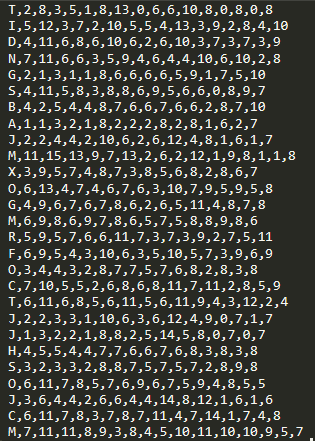
\includegraphics[width=0.5\textwidth]{data.png}
\caption{\label{fig:frog}Data Format for Test 1}
\end{figure}
\subsubsection{Hyperparameter}
Users can modify three Hyperparameters while using MLP library. In test 1, hidden layer size, iteration times, learning rate were set as following. Activate function is sigmod function.
\begin{table}[H]
\centering
\begin{tabular}{|c|c|}
 \hline
Hyperparameter& Value \\
 \hline
Hidden Layer Size & 5   \\
 \hline
Learning Rate& 0.1(fixed)\\
  \hline
Iteration times & 200\\
\hline
\end{tabular}\\
\caption{\label{tab:widgets}Hyperparameters for Test 1}
\end{table}
\subsubsection{Test Result}
After training, the MLP model reaches an accuracy of 91.45\% in classifying "O" and "D" and an accuracy of 96.32\% in classifying "O" and "X".
\begin{figure}[H]
\centering
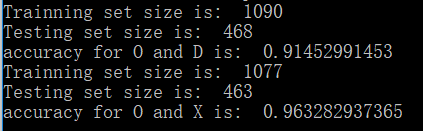
\includegraphics[width=0.5\textwidth]{res1.png}
\caption{\label{fig:frog}Data Format for Test 1}
\end{figure}
\subsection{Test 2}
\subsubsection{Data Format}
Test 2 uses stock data download from \url{https://challenger.ai/competition/trendsense/subject}. Test uses 87 features and provided label for every piece of data. Label "0" stands for not worth to buy while label "1" stands for worth to buy.
\subsubsection{Hyperparameter}
In test 2, hidden layer size, iteration times, learning rate were set as following. Activate function is sigmod function.
\begin{table}[H]
\centering
\begin{tabular}{|c|c|}
 \hline
Hyperparameter& Value \\
 \hline
Hidden Layer Size & 55   \\
 \hline
Learning Rate& 0.1(fixed)\\
  \hline
Iteration times & 200\\
\hline
\end{tabular}\\
\caption{\label{tab:widgets}Hyperparameters for Test 2}
\end{table}
\subsubsection{Test Result}
After training, the MLP model reaches an accuracy of 66.66\% in classifying "worth to buy" and "not worth to buy".
\begin{figure}[H]
\begin{minipage}[t]{0.5\textwidth}
\centering
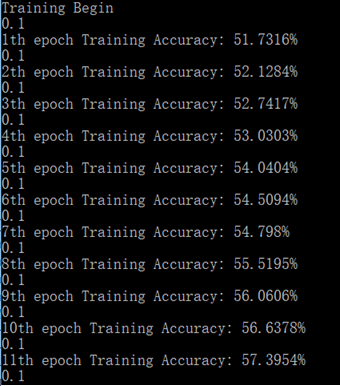
\includegraphics[width=2.2in,height=2.5in]{pro.png}
\caption{Training Log}
\label{fig:side:a}
\end{minipage}%
\begin{minipage}[t]{0.5\textwidth}
\centering
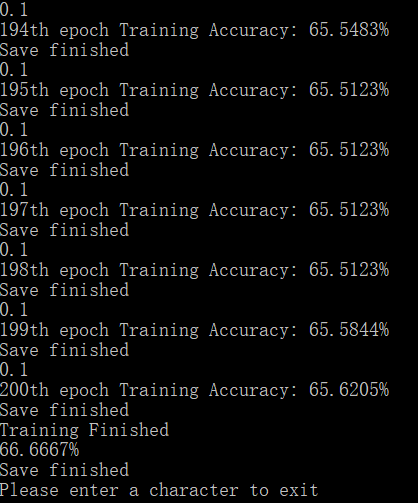
\includegraphics[width=2.1in,height=2.5in]{res.png}
\caption{Result Log}
\label{fig:side:b}
\end{minipage}
\end{figure} 
\subsection{Summary}
The hyperparameters used in the test 2 can not be asserted as optimal. It may takes a lot time to find out the best combination of Hyperparameters. This is definitely not the ultimate goal to implement these libraries. The goal is providing an useful tool for data analysis and classification in finance engineering field. Two tests above show the usability and flexibility of the MLP library, fulfilling the goal.
\section{Conclusion}
In this project, we successfully implemented a usable and flexible MLP library and its dependent libraries in C++. The test results shows its ability to express and solve finance engineer problems. 








\newpage
\begin{thebibliography}{9}
\bibitem{nano3}
 Bishop, C. M. (2006), Pattern Recognition and Machine Learning, Springer, ISBN 978-0-387-31073-2
\bibitem{nano2}
 NumPy official website http://www.numpy.org/
\bibitem{nano1} 
 "What is an Activation Function?". deepai.org https://deepai.org/machine-learning-glossary-and-terms/activation-function
\bibitem{nano4}
 Nair, Vinod; Hinton, Geoffrey E. (2010), "Rectified Linear Units Improve Restricted Boltzmann Machines", 27th International Conference on International Conference on Machine Learning, ICML'10, USA: Omnipress, pp. 807–814, ISBN 9781605589077
\bibitem{nano5} 
  He, Kaiming; Zhang, Xiangyu; Ren, Shaoqing; Sun, Jian (2015-02-06). "Delving Deep into Rectifiers: Surpassing Human-Level Performance on ImageNet Classification". arXiv:1502.01852 
\bibitem{nano6} 
 Clevert, Djork-Arné; Unterthiner, Thomas; Hochreiter, Sepp (2015-11-23). "Fast and Accurate Deep Network Learning by Exponential Linear Units (ELUs)". arXiv:1511.07289
\bibitem{nano7}
 Rosenblatt, Frank. x. Principles of Neurodynamics: Perceptrons and the Theory of Brain Mechanisms. Spartan Books, Washington DC, 1961
\bibitem{nano8}
 Rumelhart, David E., Geoffrey E. Hinton, and R. J. Williams. "Learning Internal Representations by Error Propagation". David E. Rumelhart, James L. McClelland, and the PDP research group. (editors), Parallel distributed processing: Explorations in the microstructure of cognition, Volume 1: Foundation. MIT Press, 1986.
\bibitem{nano9}
 Cybenko, G. 1989. Approximation by superpositions of a sigmoidal function Mathematics of Control, Signals, and Systems, 2(4), 303–314.
\end{thebibliography}
\end{document}